\documentclass[11pt,letterpaper]{article}
\usepackage[margin=2cm]{geometry}
\usepackage{amsmath,amssymb,graphicx,xcolor,booktabs,tabularx,enumitem,titlesec,fancyhdr,array,longtable}
\usepackage{tikz}
\usetikzlibrary{arrows.meta,positioning,shapes.geometric,fit,calc,decorations.pathreplacing}
\usepackage[hidelinks]{hyperref}
\usepackage{helvet}\renewcommand{\familydefault}{\sfdefault}
\usepackage{caption}
\titleformat{\section}{\Large\bfseries\color{blue!50!black}}{\thesection}{0.6em}{}
\titleformat{\subsection}{\large\bfseries}{\thesubsection}{0.6em}{}
\titleformat{\subsubsection}{\normalsize\bfseries}{\thesubsubsection}{0.6em}{}
\setlength{\headheight}{14pt}
\setlist{itemsep=1pt,topsep=3pt}
\setlength{\emergencystretch}{3em}
\setlength{\parskip}{3pt}
\newcommand{\boxit}[4]{\par\medskip\noindent\fcolorbox{#1}{#2}{\begin{minipage}{0.955\linewidth}\textbf{#3}\par\smallskip #4\end{minipage}}\par\medskip}
\newcommand{\conceptbox}[2]{\boxit{blue!50!black}{blue!4}{#1}{#2}}
\newcommand{\connectbox}[1]{\boxit{green!40!black}{green!5}{Connect to your analysis}{#1}}
\newcommand{\pitfallbox}[1]{\boxit{red!60!black}{red!4}{Pitfalls}{#1}}
\newcommand{\checksbox}[1]{\boxit{orange!70!black}{orange!6}{Checks}{#1}}
\newcommand{\goal}[1]{\par\noindent\textbf{Goal.} #1\par}
\newcommand{\exbox}[2]{\boxit{gray!60!black}{gray!6}{Optional exercise #1}{#2}}
\pagestyle{fancy}\fancyhf{}\lhead{sPHENIX Self-Paced Course}\rhead{Module 7: Calorimeter Reconstruction}\cfoot{\thepage}
\begin{document}
\begin{center}
{\LARGE\bfseries sPHENIX Self-Paced Course --- Module 7:}\\[4pt]
{\Large\bfseries Calorimeter reconstruction and calibration: towers, clusters, photons, jets}\\[8pt]
November 2026 \quad Prepared for P.\,D.\ Lewis (Ohio University)\\[2pt]
\small Self-contained study text based on the Summer-2026 sPHENIX School, public sPHENIX documents and standard textbook material
\end{center}

\tableofcontents
\newpage

\section*{How to use this module}
\addcontentsline{toc}{section}{How to use this module}
This module is self-contained: everything you need is in the text, and the school talks are listed only as sources.
You already know EMCal $\pi^0$ and $\eta$ reconstruction well, so this module goes beyond the basics.
It explains the reasoning behind each step of the chain, derives the formulas you use, and covers the parts of the calorimeter world you touch less often:
waveform fitting, status flags, HCal calibration, topological clustering, photon identification and jets.

\subsection*{Learning objectives}
\begin{enumerate}[label=O\arabic*.]
\item Explain how a digitised SiPM waveform becomes a calibrated \texttt{TowerInfo} entry, including zero suppression, fit quality and timing.
\item Explain each bit of the tower status word and how hot, cold and bad-$\chi^2$ towers are found.
\item Derive and critique the EMCal $\pi^0$ tower-by-tower calibration and the tower-slope method, including the absolute-scale problem.
\item Describe the HCal calibration chain (cosmic MIPs, tower slope, temperature, special corrections) and its validation.
\item Compare template clustering (\texttt{RawClusterBuilderTemplate}) with topological clustering (\texttt{RawClusterBuilderTopo}), and know when to use each.
\item Explain photon identification with shower shapes, non-collision background, isolation, and the ABCD purity method.
\item Explain calorimeter jet reconstruction: inputs, anti-$k_T$, JES/JER, in situ and data-driven checks, and underlying-event subtraction in Au+Au.
\end{enumerate}

\subsection*{Prerequisites}
Module 3 (calorimeter hardware), Module 6 (Fun4All, node tree, CDB, simulation).

\subsection*{Estimated time}
About 10--12 hours of reading; 3--4 hours for the optional exercises.

\subsection*{Sources (school talks, sPHENIX School 2026)}
\begin{itemize}
\item {[S15]} B.~Seidlitz, ``EMCal Reco and Calibrations''.
\item {[S16]} A.~Menon, ``HCal Reco and Calibrations''.
\item {[S24]} A.~C.~Oliveira da Silva, ``Topo Clustering''.
\item {[S17]} Y.~Go, ``Photon Reconstruction''.
\item {[S18]} V.~Bailey, ``Jet Reconstruction''.
\item {[S42]} A.~M.~Khan, ``HCal Calibration studies (flash)''.
\item Also consulted: {[S43]} J.~Park, ``Jet Analysis''; {[S09]} C.~Woody, ``EMCal Overview''; {[S30]} J.~Hwang, ``Transverse single-spin asymmetries of isolated prompt photons (flash)''.
\end{itemize}

\subsection*{Public readings (optional)}
Isolated prompt photons in $p$+$p$ [R1]; dijet imbalance [R2]; transverse energy density in Au+Au [R3]; calorimeter prototypes [R4]; anti-$k_T$ and FastJet [R5, R6].

\conceptbox{Conventions}{Energies are in GeV. ``Tower'' means one readout channel of a calorimeter. ``Status'' means the 8-bit word stored with each tower.
Example code fragments are written for this text; numbers quoted from public macros are labelled as such and may change. ``Toy'' marks illustrative numbers of my own.}

%=====================================================================
\section{The calorimeter reconstruction chain at a glance}
%=====================================================================
\goal{See the whole chain once before studying each link.}

\begin{figure}[h]\centering
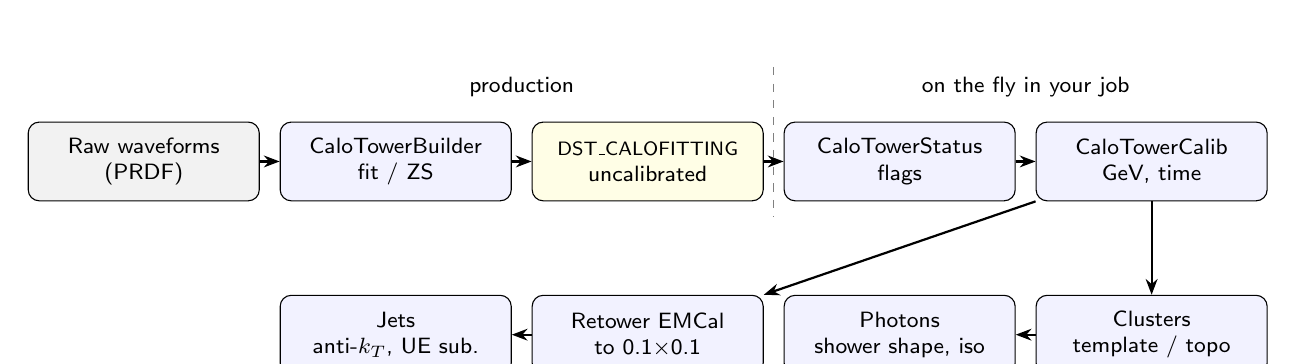
\begin{tikzpicture}[every node/.style={font=\small},
 box/.style={draw, rounded corners, text width=27mm, minimum height=10mm, align=center, fill=blue!5, font=\footnotesize},
 arr/.style={-{Stealth[length=2mm]}, thick}]
\node[box, fill=gray!10] (raw) at (0,0) {Raw waveforms\\(PRDF)};
\node[box] (fit) at (3.2,0) {CaloTowerBuilder\\fit / ZS};
\node[box, fill=yellow!10] (dst) at (6.4,0) {{\scriptsize DST\_CALOFITTING}\\uncalibrated};
\node[box] (stat) at (9.6,0) {CaloTowerStatus\\flags};
\node[box] (cal) at (12.8,0) {CaloTowerCalib\\GeV, time};
\node[box] (clu) at (12.8,-2.2) {Clusters\\template / topo};
\node[box] (pho) at (9.6,-2.2) {Photons\\shower shape, iso};
\node[box] (ret) at (6.4,-2.2) {Retower EMCal\\to 0.1$\times$0.1};
\node[box] (jet) at (3.2,-2.2) {Jets\\anti-$k_T$, UE sub.};
\draw[arr] (raw) -- (fit); \draw[arr] (fit) -- (dst); \draw[arr] (dst) -- (stat); \draw[arr] (stat) -- (cal);
\draw[arr] (cal) -- (clu); \draw[arr] (clu) -- (pho); \draw[arr] (cal.south west) -- (ret.north east); \draw[arr] (ret) -- (jet);
\node[font=\footnotesize, align=center] at (4.8,0.95) {production};
\node[font=\footnotesize, align=center] at (11.2,0.95) {on the fly in your job};
\draw[dashed, gray] (8.0,1.2) -- (8.0,-0.7);
\end{tikzpicture}
\caption{Schematic calorimeter chain (own drawing). Left of the dashed line: production; right: what \texttt{Process\_Calo\_Calib()} and later modules do in your job.}\label{fig:chain}
\end{figure}

Two facts shape everything that follows [S15]:
\begin{enumerate}
\item The production DSTs you read store \emph{uncalibrated} tower quantities (amplitude in ADC counts, time in samples, fit quality, status). Nothing else from the calorimeters is stored at that level.
\item Calibration, status flagging, clustering and all higher objects are computed on the fly in your Fun4All job. This is why a change of calibration does not require a new production.
\end{enumerate}
The node holding the fitted towers in the production DST is named per detector (for the EMCal, \texttt{TOWERS\_CEMC}); after calibration you read \texttt{TOWERINFO\_CALIB\_CEMC}.

%=====================================================================
\section{From waveform to tower}
%=====================================================================
\goal{Understand what the numbers in a \texttt{TowerInfo} mean and how reliable they are.}

\subsection{The signal}
In both the EMCal and the HCal, scintillation light is detected by SiPMs. The analog pulse is shaped and digitised by a 14-bit ADC [S15].
The digitiser samples at six times the RHIC beam clock. With the beam clock near 9.4~MHz (RHIC crossings every $\approx106$~ns), one sample lasts
\begin{equation}
\Delta t_{\mathrm{sample}} = \frac{1}{6\times 9.38\ \mathrm{MHz}} \approx 17.8\ \mathrm{ns},
\end{equation}
which matches the $\approx17.6$~ns quoted in the school [S15]. A pulse is recorded as a short train of samples (twelve to sixteen depending on detector and period).
The same digitiser electronics and the same offline processing are used for the EMCal, both HCals and the sEPD [S15].

\subsection{Template fitting}
\texttt{CaloTowerBuilder} (package \texttt{caloreco}) extracts a few numbers per tower from the samples $s_k$ [S15]. With the processing type \texttt{TEMPLATE},
it fits a measured pulse shape $T(t)$ (the template) with three free parameters:
\begin{equation}
s_k \approx P + A\,T(t_k - t_0), \qquad
\chi^2 = \sum_k \frac{\big(s_k - P - A\,T(t_k-t_0)\big)^2}{\sigma_k^2}.
\end{equation}
$A$ is the amplitude (the energy proxy), $t_0$ the peak time, $P$ the pedestal.
The fit quality is stored as $\chi^2/\mathrm{ndf}$, compressed to 8 bits on a logarithmic scale in the compact tower version [S15].
The peak time is stored as a short integer with sub-sample precision; time zero corresponds to a peak at the sixth sample [S15].
A faster non-template mode exists (\texttt{CaloWaveformProcessing::FAST}) and is used for some detectors, for example the ZDC in the public macro.

\conceptbox{Why a template, not the maximum sample?}{The maximum sample underestimates the peak when the true peak falls between samples,
and its value fluctuates with noise on one sample. A template fit uses all samples, interpolates the peak, gives a time with sub-sample resolution,
and provides a $\chi^2$ that flags distorted pulses (pile-up of two pulses, saturation, electronic glitches).}

\subsection{Zero suppression}
Fitting every channel of every event costs several seconds per event [S15]. Most towers in most events contain only noise.
The hardware therefore applies zero suppression: if the difference between a late sample (the sixth) and the first sample is below a threshold,
only those two samples are written [S15]. For such a tower:
\begin{itemize}
\item energy $=$ (sample 6) $-$ (sample 0), an integer ADC difference;
\item time and $\chi^2$ are undefined (stored as NaN);
\item the \texttt{isZS} status bit is set.
\end{itemize}
Offline, a software zero suppression can be applied before fitting to save CPU (the public \texttt{Calo\_Fitting.C} macro enables it for the EMCal and HCals), which speeds the step up by a factor of two to four [S15].
Because zero-suppressed and fully fitted towers measure amplitude differently, the calibration provides separate constants for the two cases [S15].

\pitfallbox{\begin{itemize}
\item Cutting on tower time or $\chi^2$ without handling NaN removes or keeps all zero-suppressed towers silently. Test \texttt{get\_isZS()} first.
\item Low-energy towers are mostly zero suppressed. Any per-tower timing study is therefore biased towards higher energies.
\end{itemize}}

\subsection{Tower versions}
\texttt{CaloTowerBuilder} can write different \texttt{TowerInfo} versions [S15]: \texttt{v1} (energy only), \texttt{v2} (floats for all fit outputs and the pedestal),
\texttt{v3} (\texttt{v2} plus waveform samples) and \texttt{v4} (the compact production format with an 8-bit status, packed time and compressed $\chi^2$).
Your code uses the base-class getters (\texttt{get\_energy}, \texttt{get\_time}, \texttt{get\_chi2}, \texttt{get\_status}, \dots) and works for all versions (Module 6).

\subsection{Fit performance}
Three empirical findings guide quality cuts [S15]:
\begin{itemize}
\item At low amplitude the template describes the pulses well; the noise is a few ADC counts in the HCals.
\item Some towers have distorted pulses for an entire run (huge $\chi^2$); others are distorted a small fraction of the time.
\item Both cases are caught by a $\chi^2$ cut that rises with amplitude (a fixed cut would reject good large pulses, whose $\chi^2$ grows because the template is never perfect).
\end{itemize}

%=====================================================================
\section{Tower status and hot-tower maps}
%=====================================================================
\goal{Know what each status bit means and where it comes from.}

\subsection{The status bits}
The status word holds the following flags, each with a getter in \texttt{TowerInfo} [S15]:
\par\noindent{\small
\par\noindent\begin{tabularx}{\linewidth}{@{}>{\raggedright\arraybackslash}p{0.27\linewidth}X@{}}\toprule
Getter & Meaning \\\midrule
\texttt{get\_isHot()} & Tower found hot, dead or cold in an offline map. \\
\texttt{get\_FitStatus()} & Waveform fit failed or was not performed. \\
\texttt{get\_isBadChi2()} & Fit $\chi^2$ above the amplitude-dependent threshold. \\
\texttt{get\_isNotInstr()} & Channel missing at tower building (not instrumented or not read out). \\
\texttt{get\_isNoCalib()} & No calibration constant for this channel. \\
\texttt{get\_isZS()} & Zero suppressed (two samples only). \\
\texttt{get\_isRecovered()} & Recovered by a rare procedure that repairs a flipped bit in the data. \\
\texttt{get\_isSaturated()} & Waveform reached the ADC maximum. \\
\texttt{get\_isGood()} & Convenience: none of the disqualifying flags is set (check the current source for which flags enter). \\\bottomrule
\end{tabularx}}

\subsection{How hot and cold towers are found}
A hot tower fires too often or with too much energy; a cold tower too rarely; a dead tower never.
Because the detector is symmetric in azimuth, towers at the same $\eta$ should behave alike.
The offline procedure compares each tower's hit frequency (or summed energy) with the other towers in its $\eta$ ring and flags $5\sigma$ outliers [S15].
In \texttt{CaloTowerStatus} this appears as a $z$-score threshold.
The flags are stored per run in the CDB and applied on the fly. A global hot map (towers bad in many runs) can be applied in addition.

\subsection{How CaloTowerStatus is configured}
The public calibration macro creates one \texttt{CaloTowerStatus} per detector and sets a time cut for flagging out-of-time towers.
Thresholds for bad $\chi^2$ are configurable as a constant plus a term growing with amplitude (setters \texttt{set\_badChi2\_const\_threshold}, \texttt{set\_badChi2\_quadratic\_threshold}, \dots).
In simulation, the data hot map is \emph{not} applied unless you request it, for example with \texttt{set\_directURL\_hotMap(...)}.

\subsection{Why status matters for physics}
\begin{itemize}
\item A hot tower creates fake high-energy clusters and fake triggers; with photon triggers it can dominate the triggered sample in a run.
\item A dead tower removes acceptance and splits showers that straddle it, biasing cluster energy and position.
\item Data and simulation must have the same acceptance: either mask the same towers in simulation, or correct for the difference.
\end{itemize}

\connectbox{Your pass 1 already fills per-run $96\times256$ maps of good and hot towers from \texttt{TOWERINFO\_CALIB\_CEMC}. These maps are exactly the
input you need to (i) build the run-averaged data acceptance, (ii) apply the same mask to your efficiency simulation (where the data hot map is
not applied by default), and (iii) find runs in which a large block of towers is missing. Weighting each run's map by its luminosity gives the
effective acceptance for the cross section.}

%=====================================================================
\section{Energy and time calibration of towers}
%=====================================================================
\goal{Understand what \texttt{CaloTowerCalib} applies and where the constants come from.}

\subsection{What is applied}
\texttt{CaloTowerCalib} converts each tower's amplitude to energy with a single multiplicative constant (one for fitted and one for zero-suppressed amplitudes),
and calibrates time by subtracting the tower's mean time over the run [S15]:
\begin{equation}
E_i = c_i\,A_i, \qquad t_i^{\mathrm{cal}} = t_i - \langle t_i\rangle_{\mathrm{run}}.
\end{equation}
For the EMCal the energy unit is defined so that the response to a single photon is one [S15]: ``1~GeV'' means ``the tower signal of a 1~GeV photon''.
For the HCal the scale is the electromagnetic scale (Section~\ref{sec:hcal}), so hadrons read low.
In simulation, an extra recalibration step can be applied on top (the public macro adds a \texttt{CaloTowerCalib} with a simulation recalibration payload).

\subsection{Timing}
Tower times are calibrated so that low-energy deposits peak at zero [S15]. The reported time shows a dependence on energy whose origin (physics or template artefact) was still under study [S15].
Timing is powerful: the time difference of the two $\pi^0$ decay photons measures the single-photon time resolution, and timing rejects out-of-time background such as beam-induced muons (Section~\ref{sec:ncb}) and cosmic rays in jet samples.
%=====================================================================
\section{EMCal calibration with neutral pions}\label{sec:pi0cal}
%=====================================================================
\goal{Derive the tower-by-tower $\pi^0$ method, understand its convergence, and see why the absolute scale is a separate problem.}

\subsection{Two separate problems}
EMCal energy calibration splits into [S15]:
\begin{enumerate}
\item \textbf{Gain balancing (relative calibration)}: make all 24\,576 towers respond equally.
\item \textbf{Absolute scale}: fix the common factor so that a photon of energy $E$ reads $E$.
\end{enumerate}
The $\pi^0\to\gamma\gamma$ peak serves both, but in different ways.

\subsection{Kinematics you will use}
For two massless photons with energies $E_1,E_2$ and opening angle $\theta_{12}$,
\begin{equation}
m_{\gamma\gamma}^2 = 2E_1E_2\,(1-\cos\theta_{12}).
\end{equation}
With the energy asymmetry $\alpha=|E_1-E_2|/(E_1+E_2)$ and $E=E_1+E_2$, one has $E_1E_2=\tfrac14E^2(1-\alpha^2)$, so
\begin{equation}
\sin\frac{\theta_{12}}{2} = \frac{m}{E\sqrt{1-\alpha^2}}, \qquad \theta_{\min}\approx\frac{2m}{E}\ \ (\alpha=0).
\end{equation}
\textbf{Worked example.} For a 10~GeV $\pi^0$, $\theta_{\min}\approx2(0.135)/10=0.027$~rad. At the EMCal inner radius of about 0.9~m (design value) the photons are separated by about 2.4~cm,
comparable to one tower ($\Delta\phi=2\pi/256\approx0.0245$~rad, i.e.\ $\approx2.2$~cm at 0.9~m). Above roughly 10~GeV the two showers increasingly overlap and must be separated by cluster splitting (Section~\ref{sec:template}).
For an $\eta$ meson the opening angle is four times larger at the same energy, which is why merging is not a problem for $\eta$ in your $p_T$ range.

\subsection{Gain balancing: the iteration}
Suppose tower $i$ has a gain error $g_i$, so that a photon whose shower is centred in tower $i$ reads $E_1^{\mathrm{meas}}=g_iE_1$.
If the partner photon is correctly measured,
\begin{equation}
m^{\mathrm{meas}} = \sqrt{g_i}\;m, \qquad\Rightarrow\qquad g_i = \left(\frac{m_i^{\mathrm{peak}}}{m_{\mathrm{ref}}}\right)^2 .
\end{equation}
The procedure therefore is:
\begin{enumerate}
\item Select photon-like clusters (energy above a threshold, good shape) and form all pairs per event. Assign each pair to the leading tower of each cluster.
\item For each tower, histogram the pair mass of the pairs assigned to it and fit the $\pi^0$ peak (Gaussian plus a smooth background).
\item Update the constant: $c_i \leftarrow c_i\,(m_{\mathrm{ref}}/m_i^{\mathrm{peak}})^{\kappa}$, with $\kappa$ between 1 and 2.
\item Recluster with the new constants and repeat until the peak positions stop moving.
\end{enumerate}
In practice the partner photon is itself measured by other, imperfectly calibrated towers, and a cluster spreads over several towers.
Each update therefore removes only part of the error, and several iterations are needed; the school showed the per-tower peaks converging after several iterations [S15].
The public package \texttt{calib\_emc\_pi0} (class \texttt{CaloCalibEmc\_Pi0}) implements the histogramming and fitting, including grouping towers into $\eta$ slices (methods with names such as \texttt{Loop}, \texttt{Fit\_Histos}, \texttt{Fit\_Histos\_Etas96}).

\conceptbox{Statistics per tower}{With 24\,576 towers, each tower needs enough pairs for a stable peak fit. If a sample yields $N$ useful pairs and each pair is used twice (once per cluster),
the average tower receives $2N/24576$ pairs. For a 1\% statistical precision on the peak position with a relative peak width of about 10\%, you need roughly
$(10\%/1\%)^2 \times (1/\mathrm{S/B\ factor})\gtrsim 100$ signal pairs per tower, i.e.\ $N$ of order millions after cuts. This is why the calibration is done with large samples and, where needed, by grouping towers (by $\eta$ ring, or with neighbours).}

\subsection{What the reference mass should be}
It is tempting to set $m_{\mathrm{ref}}=m_{\pi^0}^{\mathrm{PDG}}=134.98$~MeV. That is wrong for an absolute scale, for three reasons:
\begin{itemize}
\item \textbf{Clustering effects.} Energy below threshold and energy shared with neighbours are lost or gained; the reconstructed peak shifts.
\item \textbf{Position resolution and the opening angle} enter $m$ as well as the energies.
\item \textbf{Resolution on a steep spectrum.} You select pairs by measured energy. On a falling spectrum, upward fluctuations are over-represented, so selected clusters are on average measured high.
\end{itemize}
\textbf{Toy derivation of the last effect.} Take a true spectrum $f(E)\propto e^{-E/T}$ and Gaussian resolution $\sigma$. The true energies of clusters observed at $E_m$ have mean
$\langle E\rangle = E_m - \sigma^2/T$. For $T=0.5$~GeV and $\sigma=0.1$~GeV at $E_m=2$~GeV (toy values), the bias is $0.02$~GeV, i.e.\ 1\%; it grows if the resolution worsens.
Hence the absolute scale depends on the single-photon resolution [S15].

\subsection{Absolute scale in practice}
The sPHENIX approach [S15] is to treat simulation as the reference:
\begin{enumerate}
\item Smear the simulated cluster energies and positions until the simulated $\pi^0$ \emph{and} $\eta$ peak widths match data.
\item With matched resolution, adjust the energy scale until the simulated and measured peak \emph{positions} agree.
\end{enumerate}
Using both mesons matters: the $\eta$ is less affected by merging and has a different photon-energy distribution, so agreement at both constrains scale and resolution separately.

\subsection{Nonlinearity}
SiPMs have a finite number of pixels. At high light levels several photons hit the same pixel and are counted once, so the response saturates.
For $N_{\mathrm{pix}}$ pixels and $N_\gamma$ incident photo-electrons, a standard model is
\begin{equation}
N_{\mathrm{fired}} = N_{\mathrm{pix}}\left(1-e^{-N_\gamma/N_{\mathrm{pix}}}\right) \approx N_\gamma\left(1-\frac{N_\gamma}{2N_{\mathrm{pix}}}\right).
\end{equation}
Together with longitudinal light attenuation in the fibres, this makes the EMCal response slightly nonlinear.
The school reported that this effect was not yet in the standard sPHENIX simulation (it had been in the test-beam simulation), and that a two-parameter implementation (photo-electrons per GeV and effective pixel number) exists and requires re-digitised samples [S15].

\connectbox{This section is the heart of your peak-position question. Three consequences: (1) a data--MC difference in $\pi^0$ and $\eta$ peak positions
can come from the absolute scale, the resolution, the cut differences, or the missing nonlinearity, and they must be separated by comparing
both mesons with identical cuts and fit functions; (2) the EMCal group's standard is to put nonlinearity and the fine scale into the simulation and
leave the data cluster energies uncorrected, so a data-side correction in your analysis must be agreed with the calorimeter group; (3) the
efficiency depends on the scale only through the cluster-energy threshold and the trigger turn-on, so a residual scale difference also becomes
a $p_T$-shift systematic on the cross section ($\delta\sigma/\sigma\approx n\,\delta E/E$ for a spectrum $\propto p_T^{-n}$).}

%=====================================================================
\section{The tower-slope method}\label{sec:ts}
%=====================================================================
\goal{Derive the tower-slope method, which you studied in simulation for your M.S., and see how the HCal uses it.}

\subsection{Principle}
In a detector symmetric in $\phi$, every tower in a given $\eta$ ring sees the same true energy spectrum, averaged over many events.
A gain error $g$ stretches a tower's measured spectrum horizontally: $f_i^{\mathrm{meas}}(E)=\frac1{g_i}f(E/g_i)$.
For an exponential spectrum $f(E)\propto e^{-E/T}$, the measured slope becomes $T_i=g_iT$, so $g_i=T_i/T$.
For a general spectrum, the method builds a reference from the sum of all towers in the $\eta$ ring and fits each tower with a two-parameter function
(normalisation and gain) derived from the reference [S16, S42]:
\begin{equation}
f_i(E) = N_i\,F_{\mathrm{ref}}(E/g_i).
\end{equation}

\subsection{Why it works, and when it fails}
\begin{itemize}
\item It needs no physics peak, only many events; minimum-bias data suffice. It can therefore follow time dependence run by run.
\item It gives only \emph{relative} gains within a ring. The absolute scale must come from elsewhere (cosmics, $\pi^0$).
\item The low-energy region must be excluded: noise, pedestal fluctuations, zero suppression and trigger thresholds distort it differently for different towers [S42].
\item The symmetry assumption fails near support structures and non-uniform material (for example the HCal ``chimney'' towers), which must be excluded [S16].
\end{itemize}
A useful validation is that the tower-slope-corrected constants, averaged over towers, preserve the overall calibration [S42].

%=====================================================================
\section{HCal calibration}\label{sec:hcal}
%=====================================================================
\goal{Follow the four-step HCal calibration and its validation.}

\subsection{The detector in numbers}
Each HCal layer (inner, outer) has 32 sectors with $2\times24$ towers, giving $24\times64=1536$ towers per layer in $\Delta\eta\times\Delta\phi=0.1\times0.1$, covering $|\eta|<1.1$ [S16].
Light from scintillating tiles is collected by wavelength-shifting fibres onto SiPMs; each tower combines several tiles (four in the inner and five in the outer HCal) [S16].
There is no hadronic resonance like the $\pi^0$ to calibrate on, so the calibration uses minimum-ionising particles.

\subsection{Step 1: absolute scale from cosmic muons}
A vertical cosmic muon is a minimum-ionising particle crossing a tower along its full depth. Its deposit has a Landau-like distribution with a well-defined most probable value (MPV).
The procedure [S16]:
\begin{enumerate}
\item Select cosmic events with topological cuts that require signals above and below the tower, so that the muon crossed vertically.
\item Fit each tower's spectrum (the school used a Gamma-function fit) to get the MPV in ADC counts.
\item Simulate cosmics (with a cosmic-ray generator) through the detector and obtain the MPV in deposited MeV.
\item The ratio gives an ADC-to-energy constant per tower, at the electromagnetic scale.
\end{enumerate}

\subsection{Step 2: tower-slope corrections with beam data}
The simulation does not include all structures outside the main body of sPHENIX, so the cosmic constants carry residual non-uniformities.
The tower-slope method on beam data (Section~\ref{sec:ts}) corrects them, which removes, for example, a visible energy suppression in one $\phi$ region [S16].
Towers behind support structures and the chimney region are excluded because the symmetry assumption fails there [S16].
The flash talk [S42] showed the same method on Au+Au data split into run ranges, to check stability over time.

\subsection{Step 3: temperature corrections}
SiPM gain depends on temperature at fixed bias voltage: the breakdown voltage rises with temperature, so the overvoltage and the gain fall.
The coefficient was measured with LED data, and run-by-run temperature corrections keep the absolute scale between cosmic campaigns [S16].
\textbf{Toy example.} If the gain falls by a few percent per degree and the hall temperature drifts by 2~$^\circ$C between cosmic runs,
the uncorrected scale drifts by several percent, larger than the target calibration precision.

\subsection{Step 4: special corrections}
A few towers show signals at half (or double) the expected height in some runs because of a cable-connection problem.
They are found by looking at hit rates per tower versus run and corrected with dedicated factors for the affected run ranges [S16].

\subsection{Validation with hit rates and pile-up}
The stability check uses the number of hits per tower per event as a function of time [S16]. A gain drift changes the fraction of deposits above threshold, hence the hit rate.
The hit rate also grows with pile-up, which must be removed first.

\textbf{Worked pile-up example (toy numbers).} RHIC revolves at about 78~kHz with 111 filled bunches per ring, giving a crossing rate $f_{bc}\approx8.7$~MHz.
If the minimum-bias trigger rate (corrected for efficiency) is $R=400$~kHz, the probability of at least one collision per crossing is $p=R/f_{bc}\approx0.046$,
so $\mu=-\ln(1-p)\approx0.047$. Among crossings with at least one collision, the fraction with two or more is
\begin{equation}
\frac{1-e^{-\mu}-\mu e^{-\mu}}{1-e^{-\mu}} \approx \frac{\mu}{2} \approx 2.3\%.
\end{equation}
The school noted that a pure Poisson correction over-corrected the hit rate in one dataset, so a data-driven pile-up removal was used instead [S16].
After all corrections, the hit-rate stability is converted to a gain uncertainty with the measured slope of hit rate versus gain [S16].

\subsection{Electromagnetic scale and its consequences}
Calibrating with muons sets the \emph{electromagnetic} scale. Hadronic showers produce invisible energy (nuclear binding, neutrons), so $e/h>1$ for these calorimeters
and hadrons read low. Consequences: topological clusters and jets built from HCal energy read below the true hadron energy (Sections~\ref{sec:topo} and \ref{sec:jets}),
and the jet energy scale must be calibrated with simulation and checked in situ. Calibration with isolated charged hadrons ($E/p$ with tracks) is the planned next step [S16, S18].

\pitfallbox{\begin{itemize}
\item Applying a constant from one period to another without the temperature correction.
\item Using tower-slope constants near support structures.
\item Forgetting that HCal energies are at the EM scale when combining EMCal and HCal energies, for example in an isolation cone or a jet.
\end{itemize}}
%=====================================================================
\section{EMCal template clustering}\label{sec:template}
%=====================================================================
\goal{Understand every step of \texttt{RawClusterBuilderTemplate} and what its outputs mean.}

\subsection{Heritage}
The EMCal clusterizer in sPHENIX descends from the PHENIX EMCal reconstruction (the \texttt{BEmcRec} family of classes) and is wrapped in the Fun4All module \texttt{RawClusterBuilderTemplate} (package \texttt{caloreco}) [S17].
``Template'' refers to the use of a measured or simulated electromagnetic \emph{shower profile} to describe how a photon's energy spreads among towers.

\subsection{Step by step}
\begin{enumerate}
\item \textbf{Tower selection.} Take calibrated towers above an energy threshold, after status selections. The public data macro sets a threshold of 70~MeV;
the simulation macro uses 30~MeV, matched to the profile file it loads [S17].
\item \textbf{Connected groups.} Join towers that share an \emph{edge} in $(\eta,\phi)$ into parent clusters. Diagonal (corner) neighbours are not connected [S17].
\item \textbf{Local maxima.} Inside each parent cluster, find towers that are local maxima above a peak threshold (quoted as 80~MeV in the school) [S17].
\item \textbf{Splitting.} If there are several maxima, split the parent cluster: each tower's energy is shared among sub-clusters in proportion to the profile-predicted energy of each, iterating until stable [S17].
Splitting can be switched on or off (\texttt{setSubclusterSplitting}).
\item \textbf{Properties.} For each final cluster compute energy, centre of gravity, corrected position, core energy, the shower-shape $\chi^2$ and probability.
\end{enumerate}

\begin{figure}[h]\centering
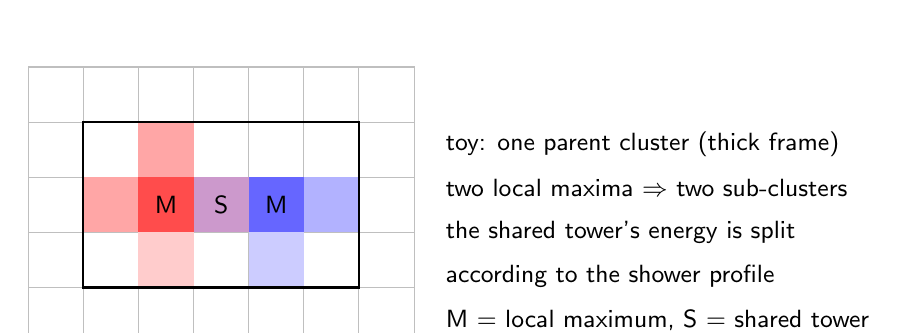
\begin{tikzpicture}[scale=0.7]
\foreach \x in {0,...,6} \foreach \y in {0,...,4} \draw[gray!50] (\x,\y) rectangle ++(1,1);
% energies (toy)
\fill[red!70] (2,2) rectangle ++(1,1); \fill[red!35] (1,2) rectangle ++(1,1); \fill[red!35] (2,3) rectangle ++(1,1); \fill[red!20] (2,1) rectangle ++(1,1);
\fill[blue!60] (4,2) rectangle ++(1,1); \fill[blue!30] (5,2) rectangle ++(1,1); \fill[blue!20] (4,1) rectangle ++(1,1);
\fill[violet!40] (3,2) rectangle ++(1,1);
\node[font=\small] at (2.5,2.5) {M}; \node[font=\small] at (4.5,2.5) {M}; \node[font=\small] at (3.5,2.5) {S};
\draw[thick] (1,1) rectangle (6,4);
\node[font=\small, anchor=west] at (7.4,3.6) {toy: one parent cluster (thick frame)};
\node[font=\small, anchor=west] at (7.4,2.8) {two local maxima $\Rightarrow$ two sub-clusters};
\node[font=\small, anchor=west] at (7.4,2.0) {the shared tower's energy is split};
\node[font=\small, anchor=west] at (7.4,1.2) {according to the shower profile};
\node[font=\small, anchor=west] at (7.4,0.4) {M = local maximum, S = shared tower};
\end{tikzpicture}
\caption{Toy illustration of parent-cluster splitting (own drawing, not data).}\label{fig:split}
\end{figure}

\subsection{Position and the shower depth}
The raw position is the energy-weighted centre of gravity (or a logarithmically weighted one, which reduces the bias towards the central tower).
Two corrections follow:
\begin{itemize}
\item \textbf{S-curve correction.} With towers comparable to the Moli\`ere radius, a linear centre of gravity is biased towards the tower centre; a correction function maps it to the true impact point.
\item \textbf{Shower depth and vertex.} The EMCal is approximately projective towards $z=0$. A shower develops to a depth $t_{\max}\propto\ln E$ along the photon direction.
For a vertex at $z_v\neq0$ the photon enters at an angle, and the measured position at shower maximum differs from the entry point. The builder can correct for depth (\texttt{set\_UseCorrectShowerDepth}) and use the event vertex from the MBD (\texttt{set\_UseAltZVertex}, which the public data macro enables) [S17].
A detailed-geometry option (\texttt{set\_UseDetailedGeometry}) uses the true tower positions rather than an idealised cylinder.
\end{itemize}
After clustering, \texttt{RawClusterPositionCorrection} can apply position-dependent energy corrections to the total and core energies.

\subsection{Shower-shape $\chi^2$ and probability}
For each cluster the builder compares the tower energies $E_k$ with the profile prediction $\hat E_k$ for a single photon at the fitted position:
\begin{equation}
\chi^2 = \sum_{k\in\mathrm{cluster}}\frac{(E_k-\hat E_k)^2}{\sigma_k^2},\qquad \sigma_k^2 = \text{(profile fluctuation)} + \text{(noise)}.
\end{equation}
A single electromagnetic shower gives small $\chi^2$. Two merged photons, hadronic showers and noise clusters give larger values.
The builder also stores a probability (\texttt{get\_prob}) derived from the $\chi^2$, and there is a merged-cluster probability field (\texttt{get\_merged\_cluster\_prob}).
The \emph{core energy} (\texttt{get\_ecore}) is the energy in the towers that the profile assigns to the core of the shower. It is less sensitive to the underlying event than the total energy,
which makes it useful in Au+Au.

\connectbox{Your cluster $\chi^2$ cut is a photon-shape cut built on this profile comparison. Three points: (1) at high $\pi^0$ $p_T$ the two photons
start to merge and the merged cluster fails the $\chi^2$ cut, so the cut efficiency for $\pi^0$s falls with $p_T$; that loss must be in your
efficiency simulation with the same clusterizer settings as in data; (2) the threshold and profile file must match (the public simulation
macro and the public data macro use different thresholds, so check what your data and MC chains actually use); (3) the $\chi^2$ uses the
noise model, so a different noise level in data and simulation changes the cut efficiency. Comparing the $\chi^2$ distribution of identified
$\pi^0$ photons (peak minus side-band) between data and simulation is the cleanest check.}

%=====================================================================
\section{Topological clustering}\label{sec:topo}
%=====================================================================
\goal{Understand the 4-2-1 topological clustering, its modes, and its use for isolation and jets.}

\subsection{Idea}
A topological cluster (``topo cluster'') groups neighbouring towers whose energies are significant compared with the noise, across calorimeter layers in three dimensions [S24].
The idea comes from ATLAS. It needs no shower template, so it works for hadrons as well as photons.

\subsection{Thresholds in units of noise}
Each calorimeter has a noise level $\sigma_{\mathrm{calo}}$ (derived from the pedestal width; the code's noise parameter is a multiple of the pedestal RMS) [S24].
Three significance thresholds define the algorithm:
\begin{align}
E_{\mathrm{seed}} &= S\,\sigma_{\mathrm{calo}} \quad (S=4 \text{ by default}),\\
E_{\mathrm{growth}} &= N\,\sigma_{\mathrm{calo}} \quad (N=2),\\
E_{\mathrm{perimeter}} &= P\,\sigma_{\mathrm{calo}} \quad (P=1).
\end{align}
\begin{enumerate}
\item \textbf{Seeds}: towers above $E_{\mathrm{seed}}$ start clusters.
\item \textbf{Growth}: neighbours above $E_{\mathrm{growth}}$ are added, and the growth continues from each added tower until no neighbour passes.
\item \textbf{Perimeter}: one final layer of neighbours above $E_{\mathrm{perimeter}}$ is added, but these do not grow further [S24].
\end{enumerate}
Neighbours are defined in $\eta$, $\phi$ and across layers (EMCal, inner HCal, outer HCal); corner neighbours can be allowed (\texttt{allow\_corner\_neighbor}).
Clusters with several local maxima above configurable energies can be split (\texttt{set\_do\_split}, \texttt{set\_minE\_local\_max}).

\textbf{Why noise units?} Signal significance, not absolute energy, determines whether a tower carries information.
Using noise units makes the same algorithm sensible for the EMCal, where noise is larger per tower, and for the inner HCal, where it is small.
The perimeter step recovers the soft tails of showers that carry a non-negligible fraction of the energy.
In a toy example from the school, a long-lived neutral kaon of a few GeV produced a seed in the outer HCal, a few growth towers in both HCal layers, and soft perimeter towers in the inner HCal; the cluster recovered most, but not all, of its energy, as expected at the EM scale [S24].

\subsection{Modes}
The module \texttt{RawClusterBuilderTopo} can run on [S24]:
\begin{itemize}
\item EMCal only, and HCal (inner+outer) separately: the choice for particle-flow reconstruction, where electromagnetic and hadronic deposits must be separated;
\item all three calorimeters together: for underlying-event studies, jets and isolation.
\end{itemize}
Clusters are stored in a \texttt{RawClusterContainer} under a configurable node name (\texttt{set\_nodename}) and are read like any other clusters.

\subsection{Energy scale and position}
Because the HCal is calibrated at the electromagnetic scale, topo clusters from hadrons read below unity [S24]. A hadronic calibration with tracks is planned.
The position is the energy-weighted average of tower positions. A subtlety: the reference point of a tower differs between detectors in the simplified geometry
(tower centre for the HCal, front face for the EMCal); using the detailed EMCal geometry, which uses the tower centre, makes them consistent [S24].

\subsection{Electromagnetic versus hadronic}
Topo clusters have no template $\chi^2$, so they cannot directly identify photons. A machine-learning classifier on EMCal cluster-shape variables (number of towers, energy fractions, widths, after logarithmic or logit transformations) can separate electromagnetic from hadronic clusters [S24].

\subsection{Template versus topo: when to use which}
\par\noindent{\small
\par\noindent\begin{tabularx}{\linewidth}{@{}>{\raggedright\arraybackslash}p{0.22\linewidth}XX@{}}\toprule
 & Template (\texttt{RawClusterBuilderTemplate}) & Topological (\texttt{RawClusterBuilderTopo}) \\\midrule
Designed for & Photons and electrons in the EMCal & Any deposit, 3D across layers \\
Thresholds & Absolute energy (tower, peak) & Multiples of noise (4-2-1) \\
Splitting & Profile-based energy sharing & Local maxima \\
Shape test & $\chi^2$ and probability vs profile & None built in (ML possible) \\
Best use & $\pi^0$, $\eta$, photon ID & Isolation energy, particle flow, UE, jets \\\bottomrule
\end{tabularx}}

\connectbox{For your photon-triggered $\eta$ and $\pi^0$ samples, template clusters remain the right objects for the photons themselves. Topo clusters
become relevant if you ever need an isolation variable (for example to study the trigger bias of the photon triggers on the event topology)
or if you compare with the isolated-photon analysis, which uses topo-cluster-based isolation (Section~\ref{sec:iso}).}

\checksbox{\begin{itemize}
\item The checkpoint exercise of this module asks you to rerun clustering with two settings (for example tower threshold, or splitting on/off) and compare cluster multiplicity and energy spectra.
Expect: a lower threshold gives more and slightly more energetic clusters; switching splitting off reduces the number of clusters at high energy and creates more large-$\chi^2$ clusters.
\item The sum of cluster energies should be close to the sum of tower energies above threshold. A large difference points to a node or threshold mismatch.
\end{itemize}}
%=====================================================================
\section{Photon reconstruction and identification}
%=====================================================================
\goal{Understand how a prompt-photon analysis turns EMCal clusters into a purity-corrected photon yield.}

\subsection{Physics of prompt photons}
Prompt photons come from the hard scattering itself [S17]:
\begin{itemize}
\item \textbf{Direct photons} from quark--gluon Compton scattering ($qg\to q\gamma$, dominant at RHIC mid-rapidity) and annihilation ($q\bar q\to g\gamma$). The Compton dominance makes them sensitive to the gluon distribution.
\item \textbf{Fragmentation photons} radiated by outgoing partons.
\end{itemize}
Photons do not interact strongly in the final state, which is why they are clean probes in $p$+$p$, of initial-state spin effects in polarised collisions [S30], and as an unmodified reference in heavy-ion collisions.
The main backgrounds are decay photons from $\pi^0$ and $\eta$ mesons, whose production rates are far larger, and jets faking photons [S17].
Two tools suppress them: \emph{shower shapes} (a high-energy $\pi^0$ gives two merged showers, broader than one photon) and \emph{isolation} (decay photons come from jets and are surrounded by other particles).
The sPHENIX isolated prompt-photon cross section in $p$+$p$ at 200~GeV is public [R1].

\subsection{Photon objects and shower shapes}
\texttt{PhotonClusterBuilder} (package \texttt{caloreco}) takes EMCal clusters above an $E_T$ threshold and stores, for each, energies in various tower regions around the cluster;
ratios are formed by the analyser [S17]. It can also compute isolation from topo clusters and evaluate a BDT score from a model file or the CDB.
The main variables [S17] are:
\begin{itemize}
\item \textbf{Core fractions} in the central $2\times2$ block with towers $E_1..E_4$: $e_{t1}=(E_1+E_2+E_3+E_4)/E$, asymmetries in $\eta$ and $\phi$ such as $(E_1+E_2-E_3-E_4)/E$, and the fraction in the diagonal corner tower.
\item \textbf{Energy ratios} $E_{i\times j}/E_{m\times n}$ of rectangular windows around the centre, for example $E_{1\times1}/E_{3\times3}$ or $E_{3\times2}/E_{3\times5}$.
\item \textbf{Widths}, the energy-weighted second moments
\begin{equation}
w_\eta = \frac{\sum_i E_i(\eta_i-\bar\eta)^2}{\sum_iE_i},
\end{equation}
and the same in $\phi$, with variants that use the integer tower index, the continuous centre of gravity, or exclude the leading tower [S17].
\end{itemize}
A merged $\pi^0$ elongates the cluster along the decay plane, increasing one width; a single photon is compact.

\subsection{Non-collision background}\label{sec:ncb}
A first look at photon-triggered data revealed clusters elongated along $\eta$ with large $w_\eta$ that simulation did not reproduce [S17].
Their timing relative to the MBD was shifted negative at positive $\eta$, which indicates particles travelling along the beam from $+z$ to $-z$:
beam-induced muons (beam halo) that shower in the EMCal parallel to the beam axis [S17].
The analysis trained a BDT to reject them, with background taken from data (early clusters without a back-to-back jet) and signal from simulation, and assigned systematic uncertainties by varying the BDT cut [S17].
\textbf{Lesson for any EMCal analysis:} out-of-time, elongated clusters at high $E_T$ are a real background in triggered data, especially for photon triggers.

\subsection{Pile-up in simulation}
In $p$+$p$, a second collision in the same crossing shifts the MBD vertex, which biases cluster $E_T$ and $\eta$ (computed with the wrong vertex) and the shower shapes.
The analysis mixed single-collision and pile-up simulation with weights computed from the mean number of collisions per crossing, separately for the two crossing-angle configurations [S17]; agreement in shower shapes improved.

\subsection{Identification}
A BDT combines shower shapes (chosen to be discriminating but only weakly correlated with isolation) with $\eta$, $E_T$ and the vertex $z$ [S17].
It is trained on photon--jet (signal) and inclusive jet (background) simulation. A ``tight'' selection is a cut on the BDT score; a ``non-tight'' band of lower scores defines a background-enriched control sample [S17].

\subsection{Isolation}\label{sec:iso}
The reconstructed isolation energy is the transverse energy in a cone around the photon minus the photon's own $E_T$:
\begin{equation}
E_T^{\mathrm{iso}} = \sum_{\Delta R<R_{\mathrm{iso}}} E_T^{\mathrm{topo/tower}} - E_T^\gamma, \qquad \Delta R=\sqrt{\Delta\eta^2+\Delta\phi^2}.
\end{equation}
Using topo clusters gives a stable, noise-robust sum [S17]. The isolation cut is often chosen to grow linearly with $E_T^\gamma$, to keep the signal efficiency roughly constant.
The simulation underestimated the isolation energy, and the analysis scaled it in simulation to match data, varying the scale for a systematic [S17].
The \texttt{ClusterIso} module (package \texttt{clusteriso}) provides cone isolation for clusters.

\subsection{Purity: the ABCD method}
Even after identification and isolation, some background remains. Define four regions [S17]:
\begin{center}\begin{tabular}{lcc}\toprule
 & isolated & non-isolated \\\midrule
tight ID & A (signal region) & B \\
non-tight ID & C & D \\\bottomrule
\end{tabular}\end{center}
If, \emph{for background}, isolation and identification are uncorrelated, then $N_A^{\mathrm{bkg}}/N_B^{\mathrm{bkg}}=N_C^{\mathrm{bkg}}/N_D^{\mathrm{bkg}}$, so
\begin{equation}
N_A^{\mathrm{sig}} = N_A - N_B\,\frac{N_C}{N_D}.
\end{equation}
Signal also leaks into B, C and D. With leakage fractions $f_X=N_X^{\mathrm{sig}}/N_A^{\mathrm{sig}}$ from simulation, the corrected equation is solved for $N_A^{\mathrm{sig}}$:
\begin{equation}
N_A^{\mathrm{sig}} = N_A - \frac{(N_B-f_BN_A^{\mathrm{sig}})(N_C-f_CN_A^{\mathrm{sig}})}{N_D-f_DN_A^{\mathrm{sig}}},
\end{equation}
a quadratic equation in $N_A^{\mathrm{sig}}$. The purity is $N_A^{\mathrm{sig}}/N_A$. Its statistical uncertainty was obtained by bootstrap, its $E_T$ dependence smoothed with a fit,
and the residual correlation between isolation and identification checked by a closure test in simulation (data-driven purity versus true purity) [S17].
The same ABCD logic is used for spin asymmetries of isolated photons: $A_N=(A_N^{\mathrm{raw}}-rA_N^{\mathrm{bkg}})/(1-r)$ with $r=1-$purity [S30].

\connectbox{The ABCD idea transfers directly to your work: any time you separate a signal with two weakly correlated variables (for example
cluster shape and isolation, or shape and timing), a sideband method gives a data-driven background estimate. The key assumption is the
\emph{background} decorrelation, which you must test, for example in simulation or in a control region. Also note that the photon analysis handles
non-collision background, pile-up and timing explicitly; with your Photon-3/4 triggered samples the same backgrounds can enter the high-$p_T$
$\pi^0$ and $\eta$ yields, typically as asymmetric pairs with one fake photon. A cluster-timing cut is a cheap check.}

%=====================================================================
\section{Jet reconstruction}\label{sec:jets}
%=====================================================================
\goal{Understand calorimeter jets in sPHENIX from inputs to calibrated, background-subtracted jets.}

\subsection{What a jet is}
A jet is the output of a jet algorithm applied to a set of inputs; it is a proxy for a scattered parton, not the parton itself [S18].
A good algorithm is infrared and collinear (IRC) safe: adding a soft particle or splitting a particle collinearly must not change the jets.
Sequential recombination algorithms satisfy this [R5, R6]. For inputs $i$ with transverse momentum $k_{t,i}$, define
\begin{equation}
d_{ij}=\min\!\left(k_{t,i}^{2p},k_{t,j}^{2p}\right)\frac{\Delta R_{ij}^2}{R^2},\qquad d_{iB}=k_{t,i}^{2p}.
\end{equation}
Repeatedly find the smallest distance: if it is a $d_{ij}$, merge $i$ and $j$; if it is a $d_{iB}$, call $i$ a jet and remove it.
$p=1$ is $k_T$ (clusters soft particles first; good for tracing splittings and for estimating backgrounds), $p=0$ Cambridge/Aachen, and $p=-1$ anti-$k_T$,
which clusters around hard particles first and gives nearly circular jets of radius $R$ [S18]. sPHENIX measured anti-$k_T$ jets with $R$ from 0.2 to 0.8 [S18].

\subsection{Inputs}
Calorimeter jets in sPHENIX use calibrated towers [S18]:
\begin{enumerate}
\item EMCal towers ($0.025\times0.025$) are \emph{retowered} to the HCal grid ($0.1\times0.1$): nominally $4\times4$ EMCal towers per HCal tower; because edges do not line up exactly, a tower spanning two retowers shares its energy by area fraction [S18].
\item Bad towers (hot, cold, dead, bad waveform) are excluded; in the public macro a retower is masked if more than half of it is masked (\texttt{RetowerCEMC::set\_frac\_cut(0.5)}).
\item Each good tower (retowered EMCal, inner HCal, outer HCal) becomes a massless pseudojet. Its pseudorapidity is corrected for the event vertex [S18]:
\begin{equation}
z_T = r_T\sinh\eta_{\mathrm{det}},\qquad \eta = \sinh^{-1}\!\left(\frac{z_T-z_{\mathrm{vtx}}}{r_T}\right),
\end{equation}
where $r_T$ is the tower radius. Then $p_T=E/\cosh\eta$, $p_x=p_T\cos\phi$, $p_y=p_T\sin\phi$, $p_z=p_T\sinh\eta$.
\end{enumerate}
\textbf{Worked example.} For an outer-HCal tower at $r_T\approx2.2$~m (toy radius) and $\eta_{\mathrm{det}}=0.5$, $z_T=2.2\sinh0.5\approx1.15$~m. For $z_{\mathrm{vtx}}=+0.3$~m,
$\eta=\sinh^{-1}(0.85/2.2)\approx0.38$. Ignoring the vertex would mis-assign $\eta$ by 0.12, more than one HCal tower.

\subsection{Software}
The public macros \texttt{NoBkgdSubJetReco.C} (retowering, tower inputs, anti-$k_T$ for several $R$) and \texttt{HIJetReco.C} (the same plus underlying-event subtraction) are the recommended entry points; calling them from your macro picks up the latest developments [S18].
They are built from the modules \texttt{RetowerCEMC}, \texttt{JetReco} with \texttt{TowerJetInput} inputs and \texttt{FastJetAlgo}, \texttt{DetermineTowerBackground}, \texttt{CopyAndSubtractJets} and, for calibration, \texttt{JetCalib}.

\subsection{Performance: JES and JER}
Match each truth jet (from generated particles) to the nearest reconstructed jet and form the response $\mathcal{R}=p_T^{\mathrm{reco}}/p_T^{\mathrm{truth}}$ [S18].
Its mean is the \emph{jet energy scale} (JES) and its relative width the \emph{jet energy resolution} (JER).
Calorimeter jets have JES below one, mostly because the HCal is calibrated at the EM scale [S18]. A simulation-based correction (as a function of $p_T$, $\eta$, vertex $z$, and possibly the EMCal energy fraction) brings JES to one.

\subsection{Data-driven checks}
Simulation-based calibration is only as good as the simulation. Two in situ checks [S18, S43]:
\begin{itemize}
\item \textbf{Photon--jet balance}: $x_{J\gamma}=p_T^{\mathrm{jet}}/p_T^\gamma$. The photon is measured precisely in the EMCal, so the data/simulation ratio of $\langle x_{J\gamma}\rangle$ tests the jet scale.
\item \textbf{Dijet or multijet balance}: compare a jet with the recoil system.
\end{itemize}
\textbf{Data-driven JER from dijet asymmetry.} Define $A_J=(p_{T,1}-p_{T,2})/(p_{T,1}+p_{T,2})$ for back-to-back dijets. If both jets have the same relative resolution $r$ and the true momenta are balanced,
$A_J\approx(\delta_1-\delta_2)/2$ with $\delta_k$ independent of variance $r^2$, so $\sigma_{A_J}=r/\sqrt2$ and
\begin{equation}
\frac{\sigma(p_T)}{p_T} = \sqrt2\,\sigma_{A_J}.
\end{equation}
Physics (radiation, hadronisation) also unbalances dijets; it is removed by subtracting the particle-level asymmetry width in quadrature [S18].
The data-driven JER came out larger than in simulation, so extra smearing is applied to simulated jets [S18]. The dijet imbalance measurement [R2] uses these techniques.
The test-beam re-analysis in Module 6 adds an energy-dependent uncertainty from the single-hadron response.

\subsection{Background in jet samples}
Calorimeter jet samples contain large non-collision backgrounds (beam halo, cosmics). A back-to-back dijet requirement and tower-level timing remove most of it [S43].

\subsection{Underlying event in heavy-ion collisions}
In central Au+Au the underlying event (UE) is large and fluctuates [S18].
\textbf{Order-of-magnitude estimate.} If the transverse energy density in central collisions is of order $dE_T/d\eta\sim600$~GeV (the order measured at RHIC [R3]), then per unit area in $(\eta,\phi)$
$\rho\approx600/(2\pi)\approx95$~GeV. An $R=0.4$ jet covers $A=\pi R^2\approx0.50$, so the UE adds about 50~GeV, twice the energy of a 25~GeV jet.
Subtraction is therefore essential, and fluctuations of this background limit the resolution [S18].

Two methods were presented [S18]:
\begin{itemize}
\item \textbf{Iterative tower subtraction} (used for the Au+Au dijet and O+O jet analyses): find seed jets (anti-$k_T$, $R=0.2$) with a cut on the maximum-to-mean constituent energy; estimate the UE per $\eta$ strip excluding seed regions,
including an azimuthal modulation $\rho(\phi)=\rho_0[1+2v_2\cos2(\phi-\Psi_2)]$; subtract from towers; repeat with seeds from subtracted jets; then run the final anti-$k_T$.
\item \textbf{Area-based subtraction}: estimate $\rho$ from $k_T$ jets excluding the two leading ones, then subtract $\rho A$ from each anti-$k_T$ jet.
\end{itemize}
Fluctuations are measured with random cones, $\delta p_T=\sum_{\mathrm{cone}}E_T-\rho A$. They broaden the JER in central events; a good subtraction leaves the JES independent of centrality [S18].

\subsection{Beyond calorimeter jets}
Tracks offer better position resolution and physically meaningful constituents but miss neutrals; particle flow combines tracks and calorimeter clusters [S18, S42].
Isolated hadrons ($E/p$) and track-based jet response ($R_{\mathrm{trk}}$) are routes to the hadronic scale [S18].

%=====================================================================
\section{Hands-on exercises on SDCC (optional, suggested)}
%=====================================================================
Suggestions only; not run while writing this text. The tutorial \texttt{CaloDataAnaRun24pp} in the \texttt{tutorials} repository is a good starting point [S16].

\exbox{E1: status census}{On 1000 events of one \texttt{DST\_CALOFITTING} segment, after \texttt{Process\_Calo\_Calib()}, count towers per status flag in the EMCal.
Plot the fraction of zero-suppressed towers versus tower energy. Confirm that time and $\chi^2$ are NaN for zero-suppressed towers.}

\exbox{E2 (checkpoint): two cluster settings}{Run \texttt{RawClusterBuilderTemplate} twice in one job with different output node names (\texttt{setOutputClusterNodeName}):
once with the default threshold and once with a higher threshold, or with splitting off. Compare cluster counts, energy spectra and $\chi^2$ distributions. Make no physics claims; describe the differences and explain them.}

\exbox{E3: topo clusters}{Add \texttt{RawClusterBuilderTopo} in EMCal-only and all-calorimeter modes. For each template cluster above 3~GeV, find the nearest EMCal topo cluster and compare energies and positions.}

\exbox{E4: tower slope (toy)}{Generate toy tower spectra $\propto e^{-E/T}$ for 64 towers with random gains of a few percent, add a low-energy threshold, and recover the gains with the reference-spectrum fit. Study how the fit range affects the bias.}

\exbox{E5: jets}{Call \texttt{NoBkgdSubJetReco.C} in a simulation macro with PYTHIA8 jets, match truth and reconstructed $R=0.4$ jets, and plot the response versus truth $p_T$.}

%=====================================================================
\section{Self-test questions}
%=====================================================================
\begin{enumerate}[label=Q\arabic*.]
\item Why are calorimeter DSTs stored uncalibrated, and what does this mean for your job?
\item What is stored for a zero-suppressed tower, and why must cuts on time or $\chi^2$ handle it explicitly?
\item Why does the bad-$\chi^2$ threshold grow with amplitude?
\item How are hot and cold towers identified, and why must the same mask be applied in simulation?
\item Derive the relation between a tower gain error and the measured $\pi^0$ peak position when only one photon hits the tower. Why is the iteration not exact in one step?
\item Give three reasons why the reconstructed $\pi^0$ peak need not be at the PDG mass.
\item Explain the tower-slope method. What does it fix, and what can it not fix?
\item List the four steps of the HCal calibration and the reason for each.
\item A 10~GeV $\pi^0$ has $\alpha=0$. Estimate the photon separation at the EMCal and compare it with the tower size.
\item What do the seed, growth and perimeter thresholds of topo clustering do, and why are they in units of noise?
\item Name two shower-shape variables and explain how a merged $\pi^0$ differs from a single photon in them.
\item Write the ABCD formula without and with signal leakage, and state the key assumption.
\item Why is the vertex needed to compute the $\eta$ of calorimeter towers for jets? Estimate the error for $z_{\mathrm{vtx}}=30$~cm.
\item Derive $\sigma(p_T)/p_T=\sqrt2\,\sigma_{A_J}$ and say what must be subtracted.
\item Estimate the UE energy in an $R=0.4$ jet in central Au+Au and name two subtraction methods.
\end{enumerate}

%=====================================================================
\section{Glossary}
%=====================================================================
\begin{longtable}{@{}p{0.25\linewidth}p{0.70\linewidth}@{}}\toprule
Term & Meaning \\\midrule\endhead
ABCD method & Data-driven background estimate using two uncorrelated variables and four regions. \\
Anti-$k_T$ & Sequential recombination jet algorithm ($p=-1$) giving circular jets. \\
Core energy (ecore) & Energy in the profile-defined core of an EMCal cluster. \\
EM scale & Calibration such that electromagnetic deposits read their true energy; hadrons read low. \\
Isolation energy & Transverse energy in a cone around a photon, minus the photon. \\
JES / JER & Mean / relative width of the jet response $p_T^{\mathrm{reco}}/p_T^{\mathrm{truth}}$. \\
MPV & Most probable value of a Landau-like MIP deposit. \\
Non-collision background & Beam-halo muons and cosmics producing clusters not from the collision. \\
Purity & Fraction of true signal in the selected sample. \\
Retowering & Summing EMCal towers onto the coarser HCal grid. \\
Shower profile & Expected fractional energy in towers around a single EM shower. \\
Status word & 8-bit flag set per tower (hot, ZS, bad $\chi^2$, \dots). \\
Template fit & Fit of a known pulse shape to waveform samples. \\
Topo cluster & Cluster grown from seed towers using noise-significance thresholds. \\
Tower slope & Relative calibration by matching tower spectra in an $\eta$ ring. \\
Underlying event & Energy not associated with the hard scattering, large in heavy-ion collisions. \\
Zero suppression & Storing only two samples for small signals. \\\bottomrule
\end{longtable}

%=====================================================================
\section*{References}
\addcontentsline{toc}{section}{References}
%=====================================================================
\subsection*{School talks (sPHENIX School 2026, BNL, July 2026)}
\begin{itemize}
\item {[S09]} C.~Woody, ``EMCal Overview''.
\item {[S15]} B.~Seidlitz, ``EMCal Reco and Calibrations''.
\item {[S16]} A.~Menon, ``HCal Reco and Calibrations''.
\item {[S17]} Y.~Go, ``Photon Reconstruction''.
\item {[S18]} V.~Bailey, ``Jet Reconstruction''.
\item {[S24]} A.~C.~Oliveira da Silva, ``Topo Clustering''.
\item {[S30]} J.~Hwang, ``Transverse single-spin asymmetries of isolated prompt photons (flash)''.
\item {[S42]} A.~M.~Khan, ``HCal Calibration studies (flash)''.
\item {[S43]} J.~Park, ``Jet Analysis''.
\end{itemize}
\subsection*{Public literature}
\begin{itemize}
\item {[R1]} sPHENIX Collaboration, ``Measurement of isolated prompt photon production in $p$+$p$ collisions at $\sqrt{s}=200$ GeV with the sPHENIX detector'', arXiv:2607.03892 (sPH-JET-2026-02).
\item {[R2]} sPHENIX Collaboration, ``Measurement of dijet transverse momentum imbalance and azimuthal acoplanarity in $p$+$p$ collisions at $\sqrt{s}=200$ GeV with the sPHENIX detector'', arXiv:2606.17184 (sPH-JET-2026-01).
\item {[R3]} sPHENIX Collaboration, ``Measurement of the transverse energy density in Au+Au collisions at $\sqrt{s_{NN}}=200$ GeV with the sPHENIX detector'', Phys.\ Rev.\ C 112 (2025) 024908, arXiv:2504.02242.
\item {[R4]} C.~A.~Aidala et al., ``Design and beam test results for the sPHENIX electromagnetic and hadronic calorimeter prototypes'', IEEE Trans.\ Nucl.\ Sci.\ 65 (2018) 2901--2919, arXiv:1704.01461.
\item {[R5]} M.~Cacciari, G.~P.~Salam, G.~Soyez, ``The anti-$k_t$ jet clustering algorithm'', JHEP 04 (2008) 063, arXiv:0802.1189.
\item {[R6]} M.~Cacciari, G.~P.~Salam, G.~Soyez, ``FastJet user manual'', Eur.\ Phys.\ J.\ C 72 (2012) 1896, arXiv:1111.6097.
\item {[R7]} sPHENIX Public Results page, \url{https://www.sphenix.bnl.gov/PublicResults}.
\end{itemize}

\appendix
%=====================================================================
\section{Answers to the self-test questions}
%=====================================================================
\begin{enumerate}[label=A\arabic*.]
\item Only fitted tower quantities (ADC amplitude, time in samples, $\chi^2$, status) are stored, so calibrations can change without reprocessing. Your job must run status flagging and calibration (\texttt{Process\_Calo\_Calib()}) with the right global tag before using energies.
\item Only two samples; energy is their difference and time and $\chi^2$ are NaN, with \texttt{isZS} set. Comparisons with NaN are always false, so a cut like \texttt{chi2<X} silently drops every zero-suppressed tower, and \texttt{!(chi2>X)} silently keeps them all.
\item The template is never perfect; the residual grows with amplitude, so a good large pulse has larger $\chi^2$ than a good small pulse. A fixed cut would reject good high-energy towers.
\item By comparing each tower's rate or energy with others in the same $\eta$ ring and flagging $5\sigma$ outliers, per run. Otherwise data and simulation have different acceptances, and the efficiency is wrong.
\item $m^2\propto E_1E_2$; if $E_1\to gE_1$ then $m\to\sqrt g\,m$, so $g=(m_i/m_{\mathrm{ref}})^2$. Not exact because the partner photon and the shared shower energy involve other, still miscalibrated towers.
\item Any three of: clustering losses and sharing; position resolution entering the opening angle; resolution bias on a falling spectrum; nonlinearity; cluster merging; residual miscalibration; background shape under the peak.
\item In a $\phi$-symmetric ring, all towers see the same spectrum; a gain stretches the spectrum horizontally, so fitting each tower to the ring reference gives relative gains. It fixes tower-to-tower and time-dependent relative gains; it cannot set the absolute scale and fails where the symmetry is broken.
\item Cosmic MIP absolute scale (EM scale per tower); tower-slope beam correction (structures missing in simulation); run-by-run temperature correction (SiPM gain drift); special half-height corrections (cable faults).
\item $\theta_{\min}\approx0.027$~rad; at $\approx0.9$~m this is $\approx2.4$~cm, about one EMCal tower. The showers overlap and splitting is needed.
\item Seeds start clusters ($4\sigma$), growth adds and propagates through significant neighbours ($2\sigma$), perimeter adds one last soft layer ($1\sigma$). Noise units make the algorithm equivalent across calorimeters with different noise.
\item For example $w_\eta$ (energy-weighted width) and $E_{3\times2}/E_{3\times5}$ or the $2\times2$ core fraction: a merged $\pi^0$ has a larger width and a smaller core fraction.
\item $N_A^{\mathrm{sig}}=N_A-N_BN_C/N_D$; with leakage, $N_A^{\mathrm{sig}}=N_A-(N_B-f_BN_A^{\mathrm{sig}})(N_C-f_CN_A^{\mathrm{sig}})/(N_D-f_DN_A^{\mathrm{sig}})$. The key assumption: for background, isolation and identification are uncorrelated.
\item Towers are fixed in space; their $\eta$ seen from the vertex depends on $z_{\mathrm{vtx}}$. For a tower at $r=2.2$~m and $\eta_{\mathrm{det}}=0$, $z_{\mathrm{vtx}}=0.3$~m gives $\eta=\sinh^{-1}(-0.3/2.2)\approx-0.14$, larger than one HCal tower.
\item $A_J\approx(\delta_1-\delta_2)/2$ with independent $\delta_k$ of variance $r^2$, so $\sigma_A=r/\sqrt2$. The physics imbalance (particle-level $A_J$ width) must be subtracted in quadrature.
\item $\rho\approx95$~GeV per unit area times $A\approx0.5$ gives $\approx50$~GeV. Iterative tower subtraction with seed exclusion and flow modulation; area-based $\rho A$ subtraction.
\end{enumerate}
\end{document}
